% \subsection{Quick Print Plugin}
\subsection{Extension Impression Rapide}

% when the revision of a section has been finalized, 
% comment out the following line:
% \updatedisclaimer

% The \toolbtntwo{quick_print}{Quick Print} Plugin allows to print the current 
% map canvas with minimal effort into PDF format. All the user needs to add 
% is a Map Title, a Map Name and the Paper Size (See
% Figure~\ref{fig:quickprint}).
L'extension \toolbtntwo{quick_print}{Impression Rapide} permet d'imprimer le cadre de
la carte actuelle avec un minimum d'effort au format PDF. Tout ce qu'a besoin
d'ajouter l'utilisateur est un titre pour la carte, un nom pour la carte et la
taille de la page (voir Figure~\ref{fig:quickprint})
 
\begin{figure}[ht]
   \begin{center}
%    \caption{Quick Print Dialog \nixcaption}\label{fig:quickprint}\smallskip
   \caption{Bo\^ite de dialogue de l'Impression Rapide
\nixcaption}\label{fig:quickprint}\smallskip
   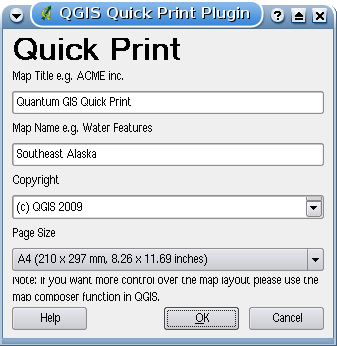
\includegraphics[clip=true, width=6cm]{quick_print_dialog}
\end{center}
\end{figure}

% Figure~\ref{fig:quickprint_result} below shows a DIN A4 quick print result 
% from the alaska sample dataset. If you want more control over the map layout, 
% please use the print composer plugin, described in
% Section~\ref{label_printcomposer}.
La figure~\ref{fig:quickprint_result} ci-dessous montre le r\'esultat de l'Impression Rapide dans un fichier A4 DIN \`a partir du jeu de donn\'ees d'\'echantillon de
l'Alaska. Si vous d\'esirez plus de contr\^ole sur la mise en page de la carte,
utiliser plut\^ot l'extension composeur de carte, d\'ecrit dans la
section~\ref{label_printcomposer}.

\begin{figure}[ht]
   \begin{center}
%    \caption{Quick Print result as DIN A4 PDF
   \caption{R\'esultat de Quick comme fichier PDF A4 DIN
\nixcaption}\label{fig:quickprint_result}\smallskip
   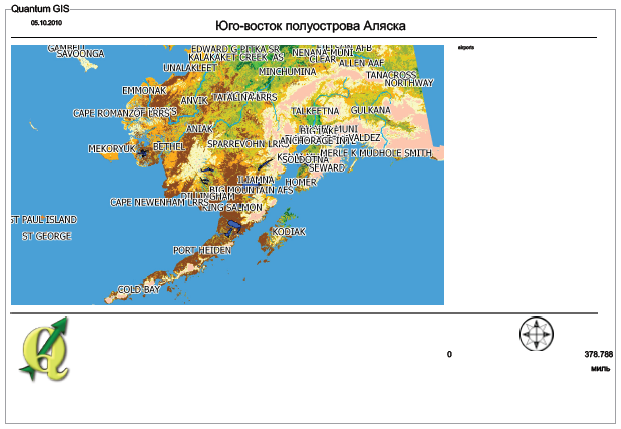
\includegraphics[clip=true, width=11cm]{quick_print_result}
\end{center}
\end{figure}